%%%%%%%%%%%%%%%%%%%%%%%%%%%%%%%%%%%%%%%%%%%%%%%%%%%%%%%%%%%%%%%%%%%%%%%%%%%%%%%%
% Author : Tomáš Vlach , Tomas Polasek (template)
% Description : Seventh exercise in the Introduction to Game Development course.
%   It deals with the creation of a Game Design Document, presenting a short 
%   pitch for a potential game project.
%%%%%%%%%%%%%%%%%%%%%%%%%%%%%%%%%%%%%%%%%%%%%%%%%%%%%%%%%%%%%%%%%%%%%%%%%%%%%%%%

\documentclass[a4paper,10pt,english]{article}

\usepackage[left=2.50cm,right=2.50cm,top=1.50cm,bottom=2.50cm]{geometry}
\usepackage[utf8]{inputenc}

% Hyper-Text References
\usepackage{hyperref}
\hypersetup{colorlinks=true, urlcolor=blue}

% Drawing Images and Graphs
\usepackage{tikz}
\usepackage{pgfplots}

% Page Utilities
\usepackage{graphicx}

% Image Sub-Captions
\usepackage{subcaption}

\newcommand{\ph}[1]{\textit{[#1]}}

\title{%
Game Pitch Document%
}
\author{%
Tomáš Vlach (xvlach24)%
}
\date{30.12.2023}

\begin{document}

\maketitle
\thispagestyle{empty}

{%
\large

\begin{itemize}

\item[] \textbf{Title:} Ascension 

\item[] \textbf{Genre:} Rogue-like

\item[] \textbf{Style:} Pixelized 3D abstract

\item[] \textbf{Platform:} PC/XBOX/PS5/Switch

\item[] \textbf{Market:} Gamers finding satisfaction in beating hard challenges 

\item[] \textbf{Elevator Pitch:} A fast-paced first-person medieval rogue-like where your life's on the line, your time is ticking and you can make it tick faster in exchange for mysterious powers.

\end{itemize}

}

\section*{\centering The Pitch}

\subsection*{Introduction}
The game shows a player the top of a mountain, their character standing down by the sea on a dock, the weapon the character wields and the timer that starts counting down to their near-inevitable doom. The player then must start their journey through progressively harder levels, unlocking more gear, trading their precious time for mysterious powers, slaying monsters to get their valuable time back and dying along the way, which brings them back to where it all began, the dock. They can try again, but now with the knowledge and new unlocked starting gear to boost them higher than before.

\subsection*{Background}
The main driving forces behind the idea for this game was several other titles like Cruelty Squad, Dead Cells, The Binding of Issac and others as well as the want to create a game where the player is not as bogged down with cut-scenes stretching for minutes, complicated menus and control schemes right out of the gate. Rather this game would try to minimize this by only having one short cut-scene at the beginning with other important events happening in-game with the player having control at all times and giving the players only basic controls to begin with and letting them then figure out how these controls combine to create more complicated outcomes by themselves. This would also mean that the game would be highly dependent on players discovering and mastering Techs ( a term for complicated inputs resulting in different outcomes ) and to incorporate them into their runs of the game.

\subsection*{Setting}
The would of Ascension is a pseudo Scandinavian medical fantasy, with folklore inspired monsters and architecture. As the players would ascend upwards they would encounter different levels with a changing landscape. For example the starting level is a fishing village down by the sea occupied by gremlins and other small creatures, the second level would be a forest just beyond the village borders occupied by more threatening enemies like trolls and giants. Other areas would be mines, castle, crypt and of course the mountain itself as last. This list is not complete and could be reworked to better suit the flow of the levels.

The player character is a newcomer to these lands so the player can swap between starting presets before starting a run of the game.

The main plot of Ascension takes a backseat to the game-play but is still represented in the world the player will explore. The village is abandoned and over run with scavengers, the forest and paths through it overgrown. The castle is over run by drauger and drakes. Only a handful of NPCs have managed to survive out here or other adventurers that came into this land to seek fortunes hidden away. It all seems to be connected with something atop the mountain. Perhaps a curse, perhaps a powerful monster or maybe something even worse then those. 

\subsection*{Features}

\begin{itemize}
  \item Quick fast-pace combat with few interruption for quicker and better game flow4
  \item Enhanced movement and combat controls for a very quick and satisfying feedback
  \item Challenge provided by not only the combat with enemies you can learn the patters to, but also by the timer that is near constantly running.
  \item The ability to sacrifice your time for powers that may help you with the rest of the run, but may also doom you in the steep price.
  \item Bosses by the end of each level that make sure you have learned the levels mechanics and gimmicks.
  \item Unlocking of new equipment for subsequent runs and be able to find the levels.
  \item Replayablility and options to add content after release.
\end{itemize}

\subsection*{Genre}

The game is a rogue-like where time and your management of it matters. The game has a first person perspective and focuses on melee combat with dodges, high mobility and understanding of your surroundings and the monsters you are fighting. It combines the time ticking action of Risk of Rain (1/2) and the satisfying combat of Dead Cells and Cruelty Squad. 

\subsection*{Platform}

The main platform this project will be aiming for is PC, but porting this game to consoles like PS5, Xbox and Switch should not be a major problem with the simple control scheme and stylized but not high-end graphics.

\subsection*{Style}

The visual style is a blend of several already existing visual styles for other games like Valheim and The Short Hike. Both example games use simple yet very understandable art-style with pixelized 3D graphics splashed with Valheim's modern visual effects added in. This project would want to create its own spin on this style and vibrant world were visual recognition would be a high priority so the player never feels like the game is to blame that they didn't see any dangers.

The locations in the game are also inspired by other modern games like for example Elden Ring or Skyrim.

\begin{figure}[h]

\centering

\begin{subfigure}{0.49\linewidth}
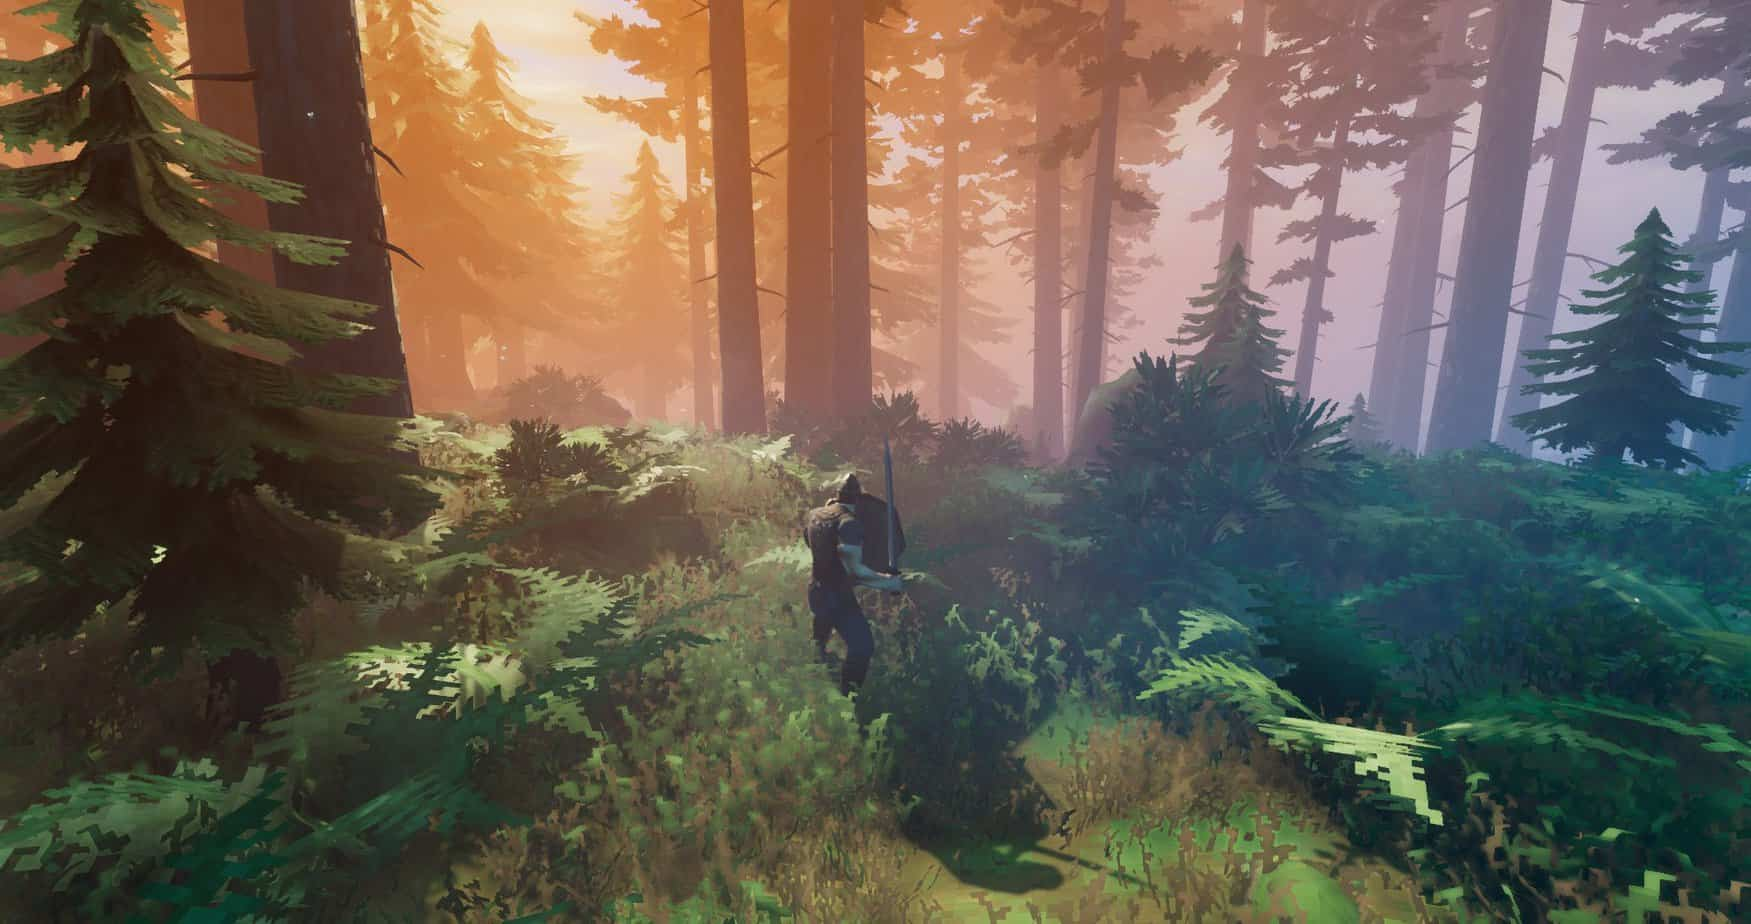
\includegraphics[width=1\linewidth]{Valheim1.jpg}
\caption{Valheim Forest}
\label{fig:valheim forest}
\end{subfigure}\hfill
%
\begin{subfigure}{0.49\linewidth}
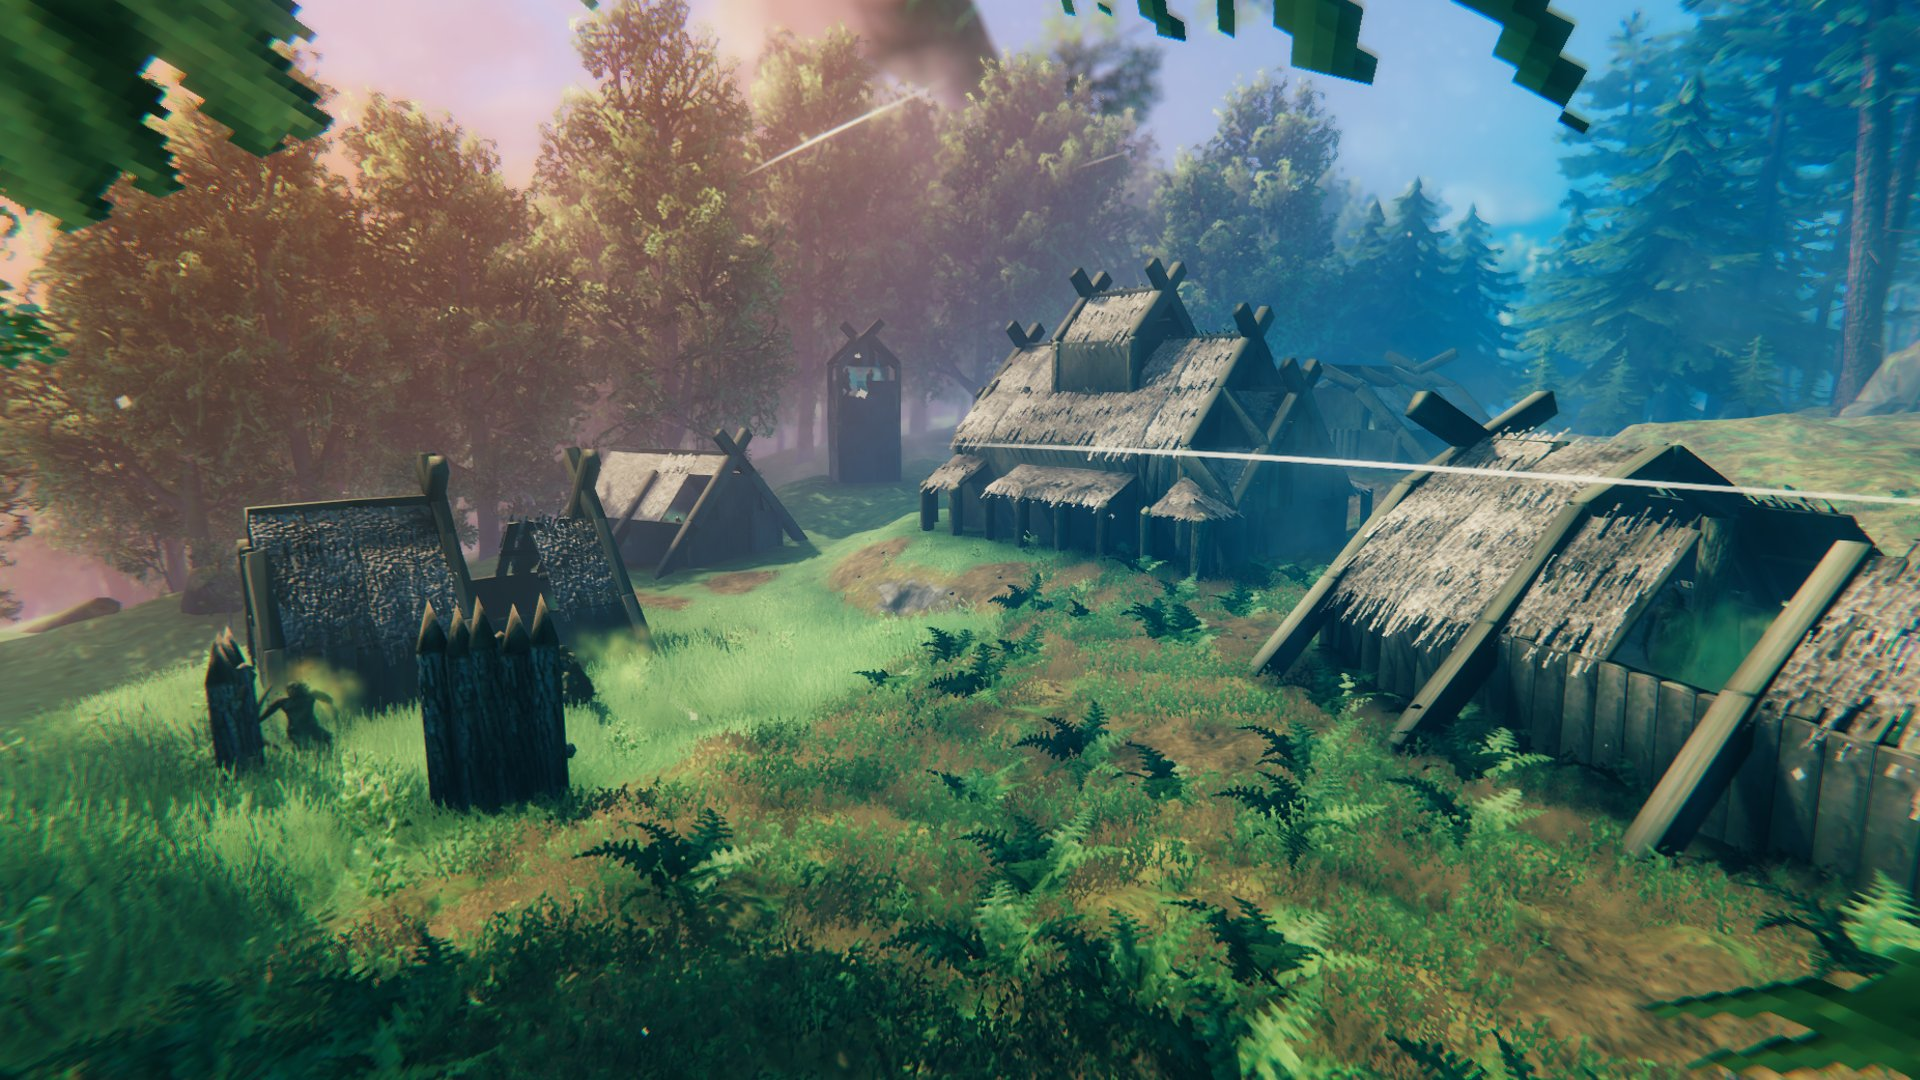
\includegraphics[width=1\linewidth]{Valheim2.jpg}
\caption{Valheim Village}
\label{fig:valheim village}
\end{subfigure}\hfill

\end{figure}

\begin{figure}[h]

\centering

\begin{subfigure}{0.49\linewidth}
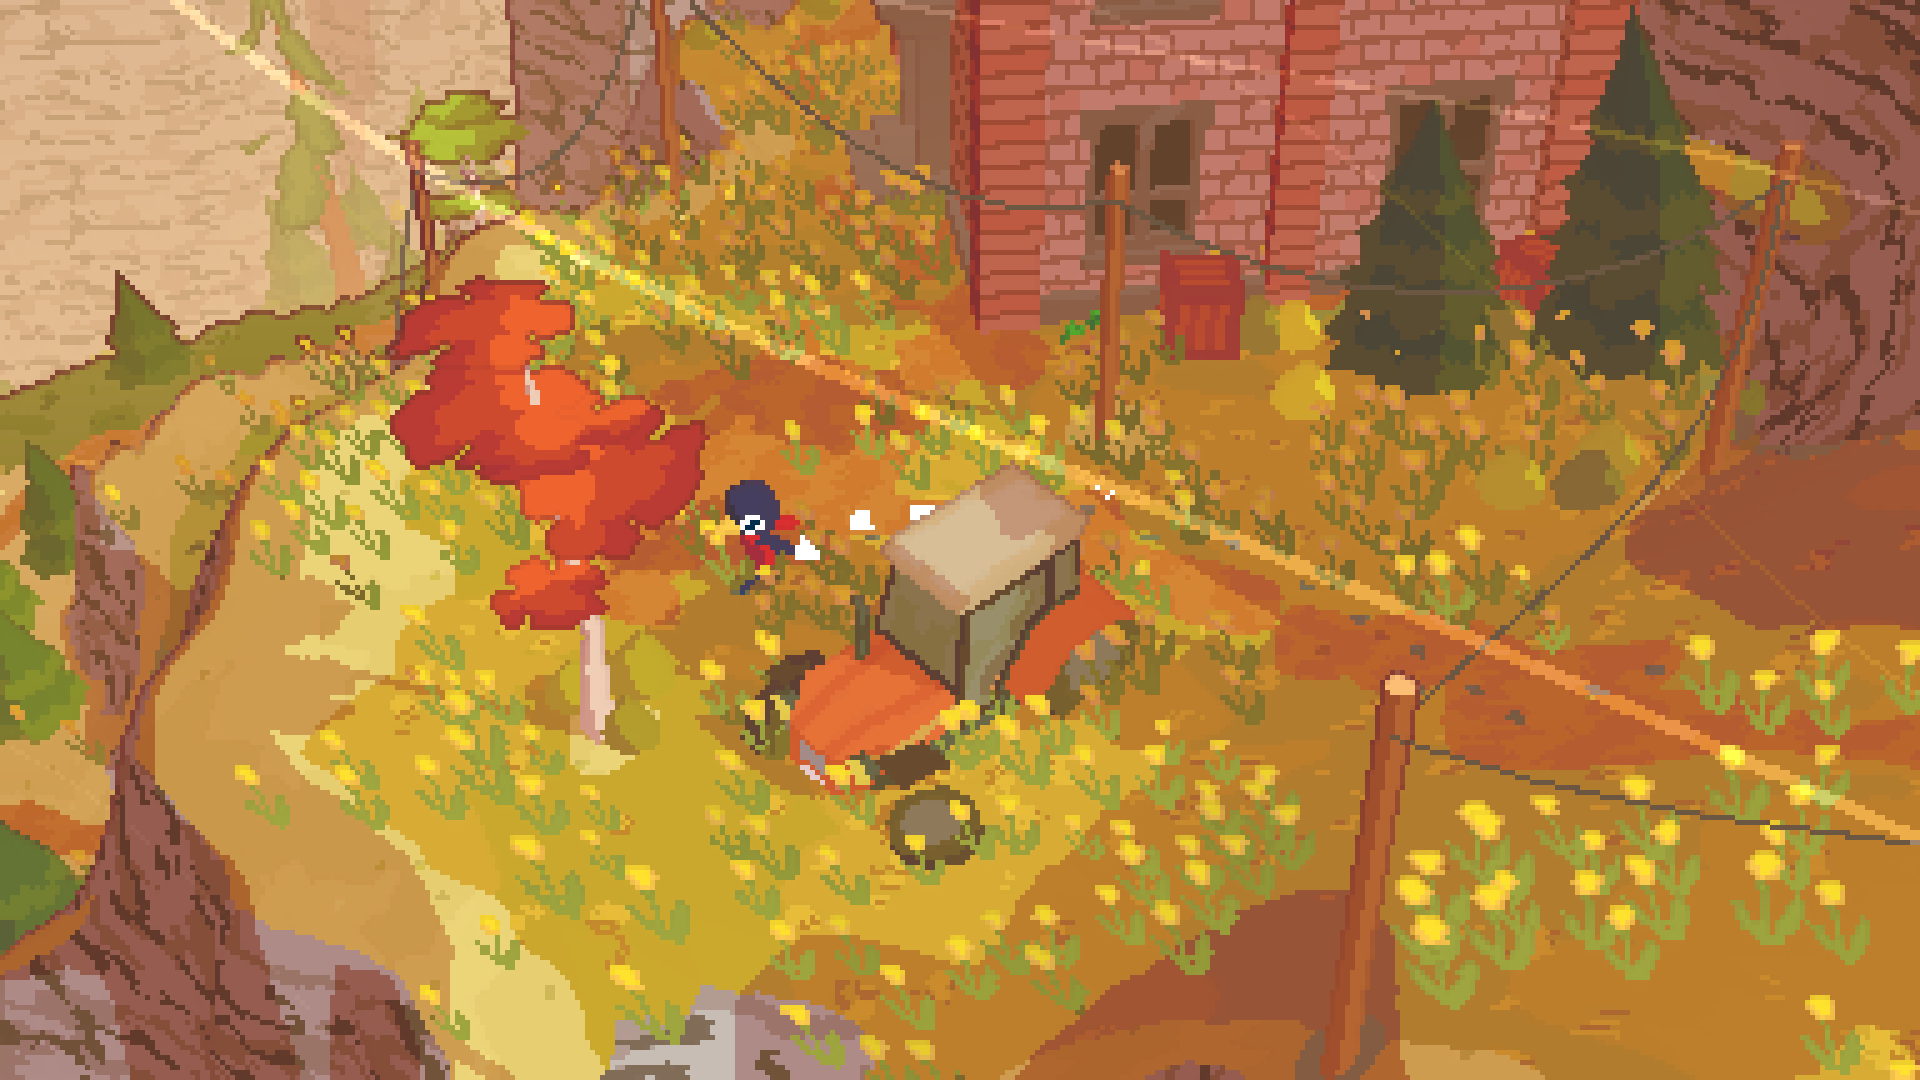
\includegraphics[width=1\linewidth]{TheShortHike1.png}
\caption{The Short Hike Meadow}
\label{fig:the short hike meadow}
\end{subfigure}\hfill
%
\begin{subfigure}{0.49\linewidth}
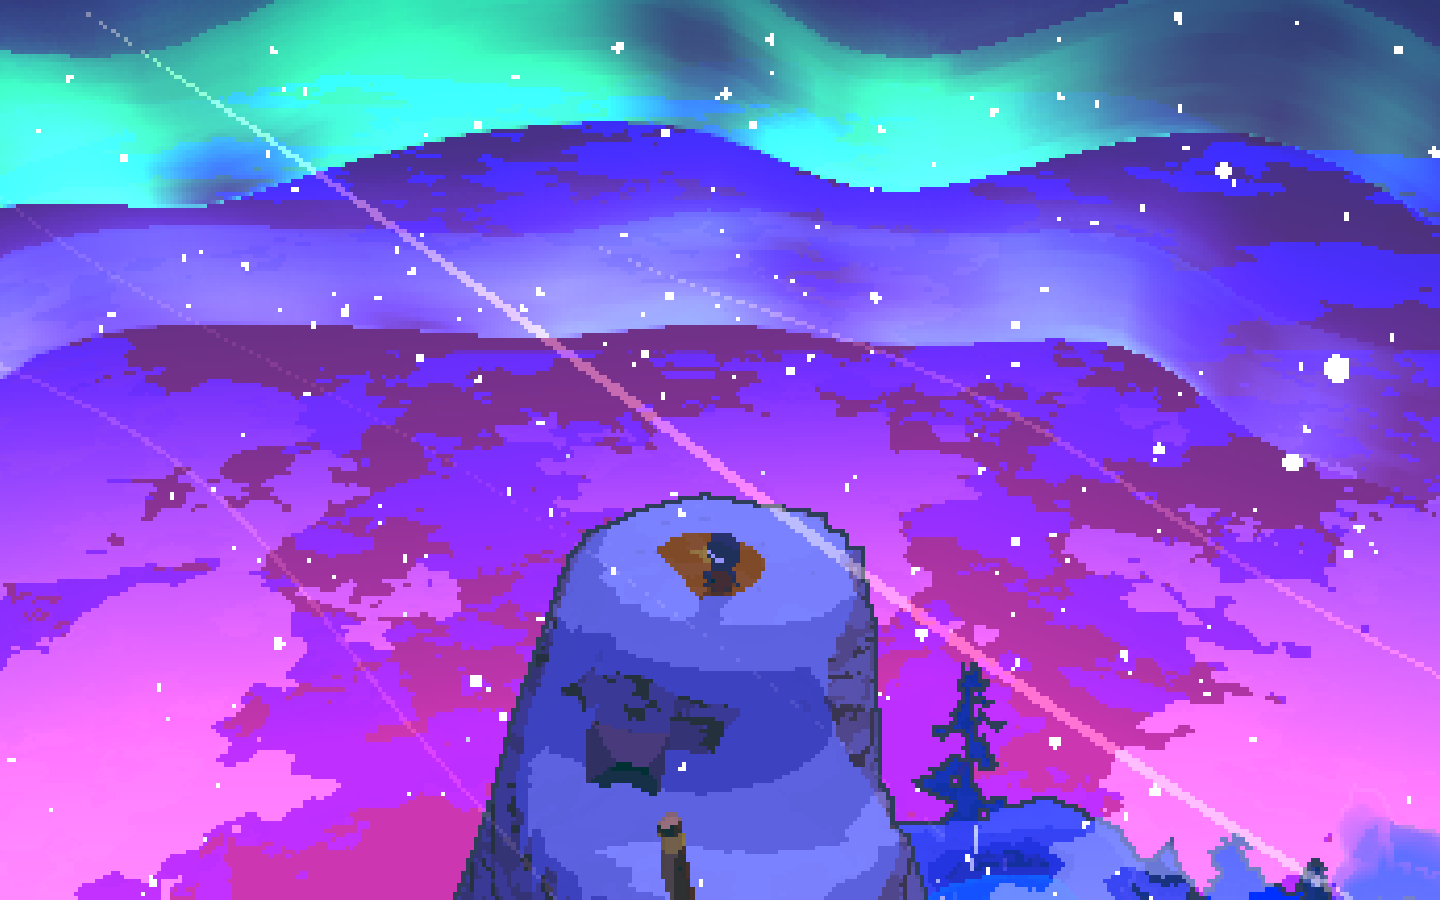
\includegraphics[width=1\linewidth]{TheShortHike2.png}
\caption{The Short Hike Mountain}
\label{fig:the short hike mountain}
\end{subfigure}\hfill

\end{figure}

\begin{figure}[h]

\centering

\begin{subfigure}{0.49\linewidth}
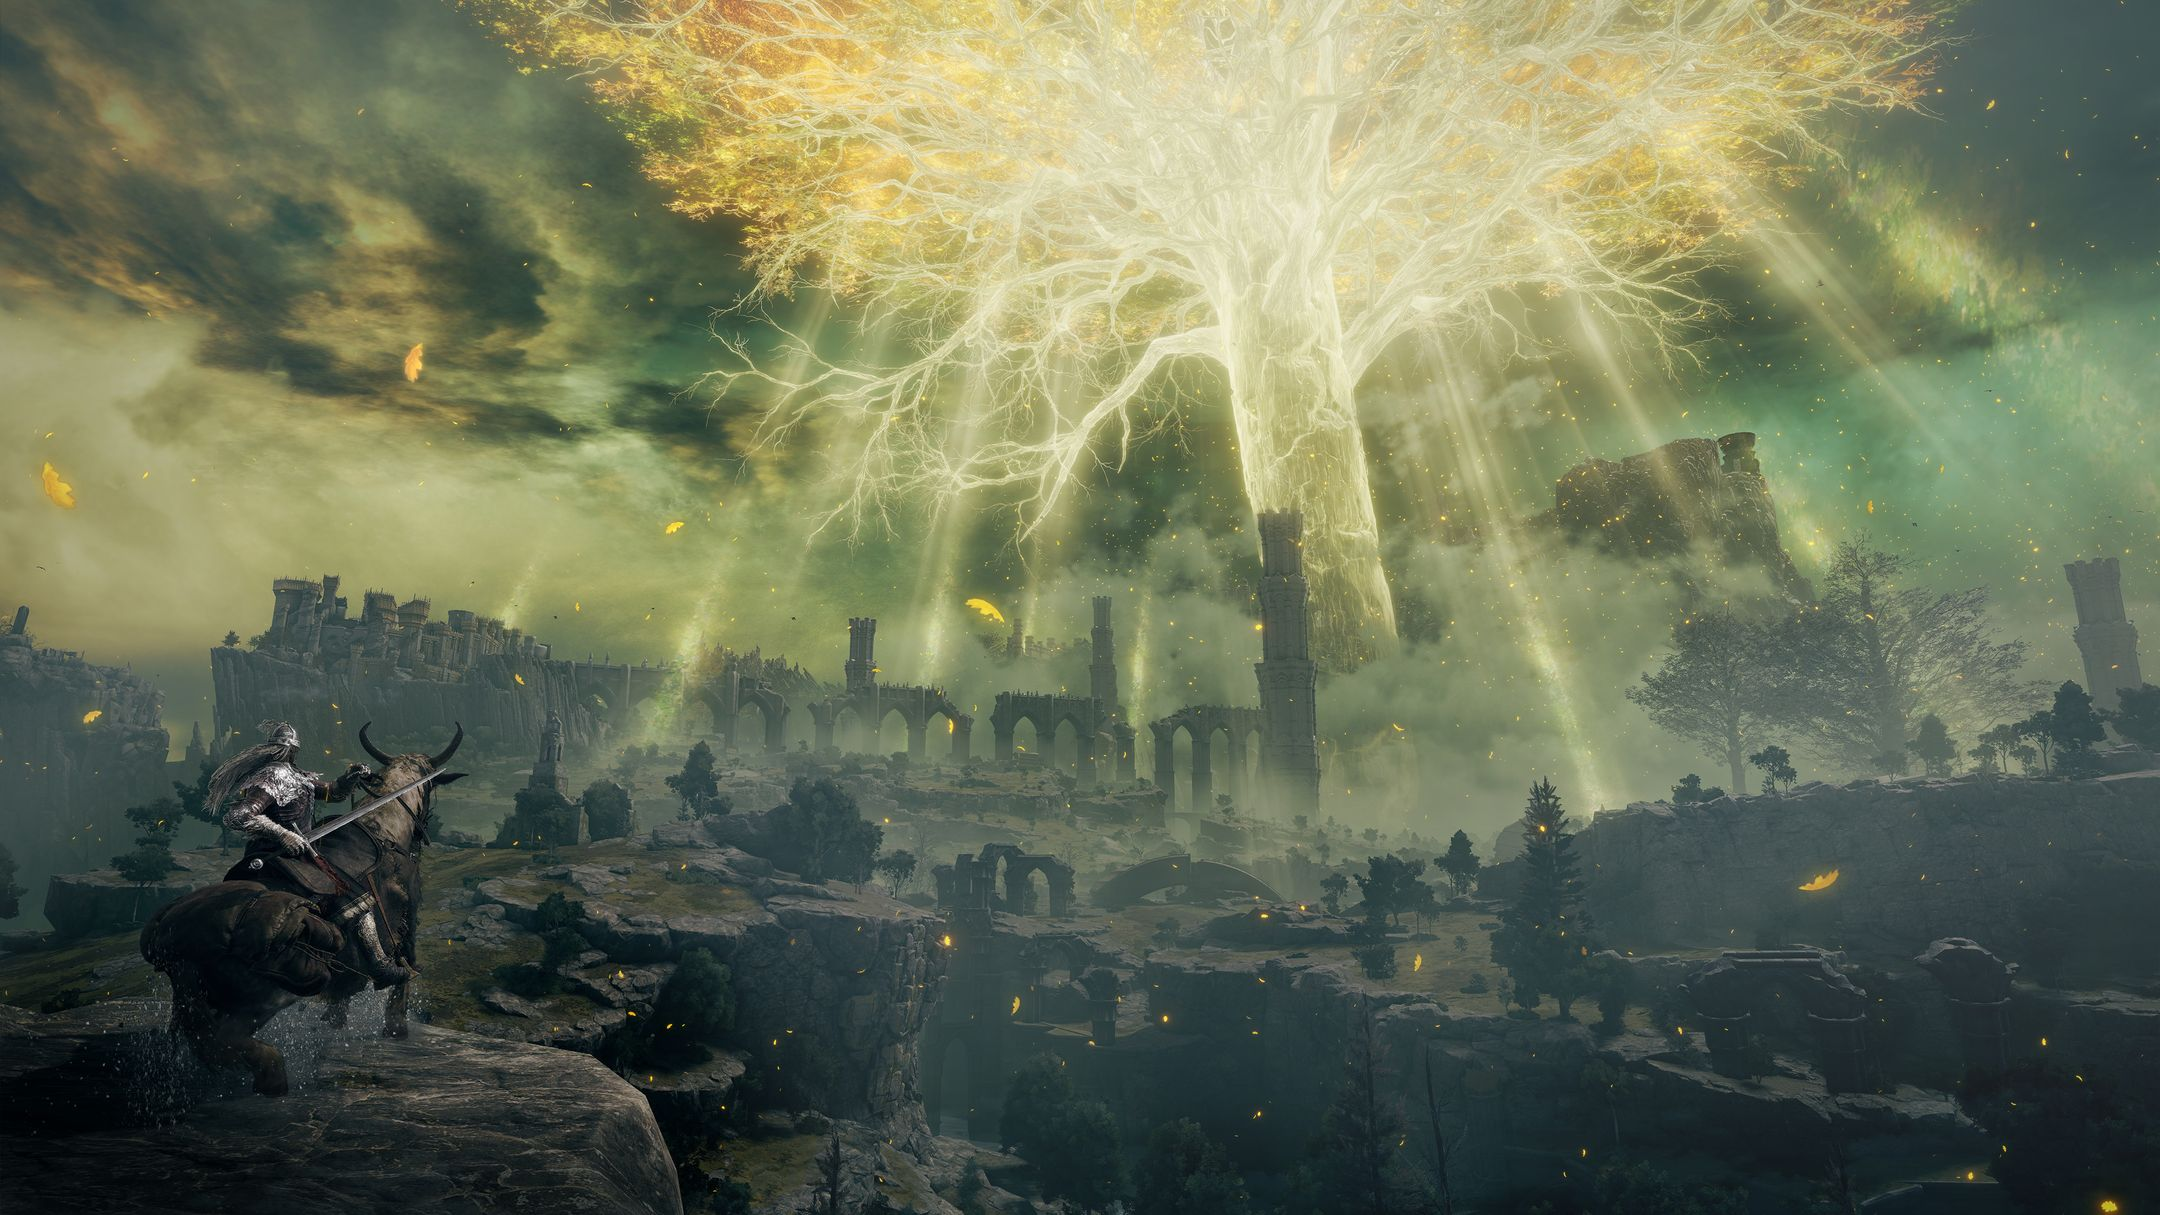
\includegraphics[width=1\linewidth]{EldenRing.jpg}
\caption{Elden Ring}
\label{fig:elden ring}
\end{subfigure}\hfill
%
\begin{subfigure}{0.49\linewidth}
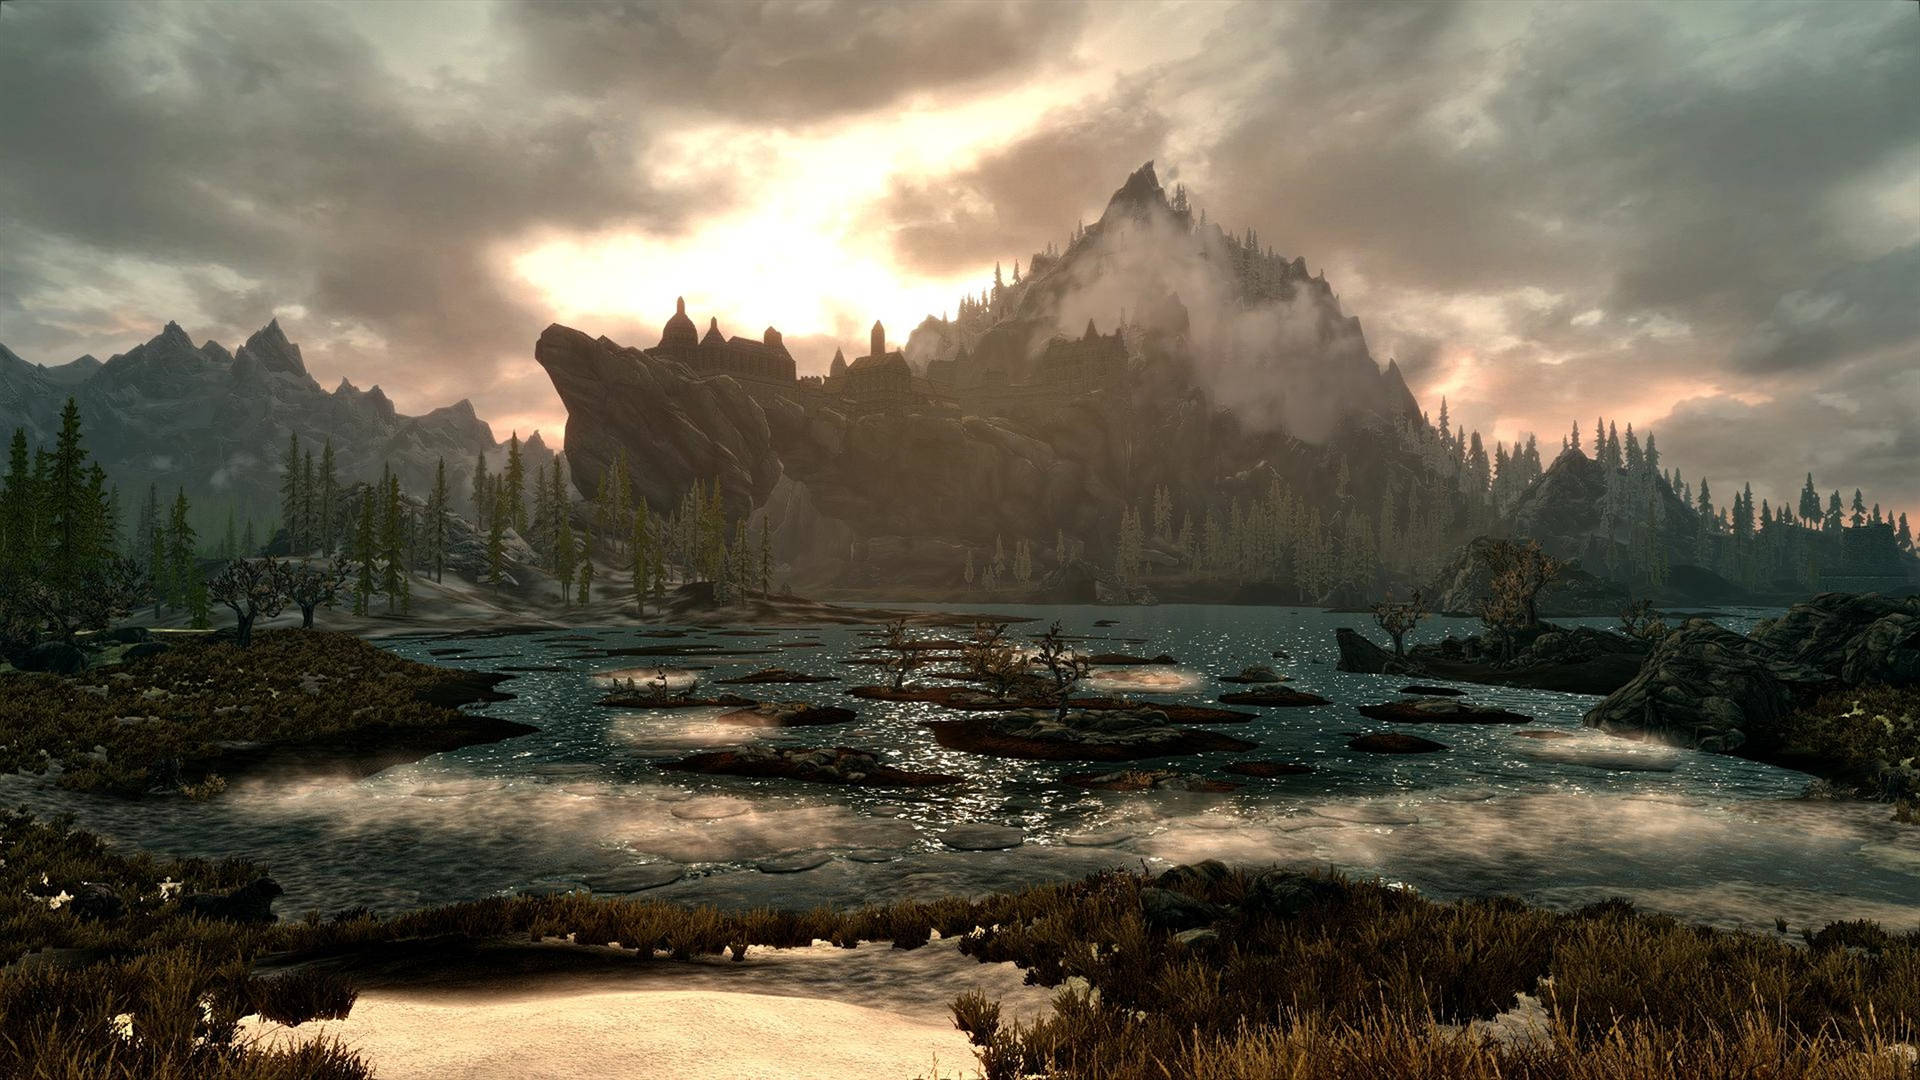
\includegraphics[width=1\linewidth]{Skyrim.jpg}
\caption{Skyrim}
\label{fig:skyrim}
\end{subfigure}\hfill

\end{figure}

\end{document}
